\documentclass{article}%
\usepackage[T1]{fontenc}%
\usepackage[utf8]{inputenc}%
\usepackage{lmodern}%
\usepackage{textcomp}%
\usepackage{lastpage}%
%
\usepackage{amsmath}%
\usepackage{amssymb}%
\usepackage{amsfonts}%
\usepackage{graphicx}%
\usepackage{hyperref}%
\usepackage{tikz}%
\usepackage{pgfplots}%
\usetikzlibrary{math}%
\title{IME 2026 - Física\thanks{This exam was solved and automatically generated with gpt-resolve: \url{https://github.com/lgabs/gpt-resolve}}}%
\author{claude{-}opus{-}5{-}5 (solver) + claude{-}opus{-}5{-}5 (judge)}%
\date{November 10, 2026}%
%
\begin{document}%
\normalsize%
\maketitle%
\section*{Questão 1}

\section*{Solução}

\textbf{Preliminares.} A força é conservativa, com $F=-\dfrac{dE_p}{dx}=-(4x-x^2)=-4x+x^2$, coerente com o enunciado (SI: $E_p$ em J, $F$ em N, $x$ em m). Como só ela atua, a energia mecânica se conserva:
\[
E=\frac{mv^2}{2}+E_p(x)\ \Longrightarrow\ \frac{mv^2}{2}=E-E_p(x)\ge 0 ,
\]
logo a partícula só ocupa posições com $E_p(x)\le E$, e os pontos de retorno ($v=0$) satisfazem $E_p(x)=E$.

Equilíbrios ($F=0$): $x(x-4)=0\Rightarrow x=0$ ou $x=4$. Como $E_p''(x)=4-2x$:
$x=0$ é mínimo ($E_p''=4>0$, estável), com $E_p(0)=0$; $x=4$ é máximo ($E_p''=-4<0$, instável), com
$E_p(4)=32-\frac{64}{3}=\frac{32}{3}$ J. Além disso, $E_p'(x)=x(4-x)$: $E_p$ decresce para $x<0$, cresce em $0<x<4$ e decresce para $x>4$.

\textbf{a)} O movimento é oscilatório quando a partícula fica presa no poço em torno de $x=0$, indo e voltando entre dois pontos de retorno $x_a<0<x_b$. À direita o poço é limitado pelo máximo ($x=4$, altura $32/3$ J); à esquerda, pelo ponto em que a curva volta a essa altura:
\[
2x^2-\frac{x^3}{3}=\frac{32}{3}\iff x^3-6x^2+32=0\iff (x-4)^2(x+2)=0\ \Longrightarrow\ x=-2 .
\]
Para $0<E<\frac{32}{3}$ J, pela monotonicidade de $E_p$, os pontos de retorno satisfazem $-2<x_a<0<x_b<4$. Os extremos ficam excluídos: só seriam atingidos com $E=\frac{32}{3}$ J, caso em que a partícula tende ao equilíbrio instável $x=4$ sem retornar (perto de $x=4$, $E-E_p\approx 2(x-4)^2$, logo $|\dot x|\propto|x-4|$ e a aproximação dura tempo infinito). Para $x<-2$ seria $E_p>\frac{32}{3}$ J, e para $x>4$ a partícula está fora da barreira e escapa ($F>0$). Assim,
\[
\boxed{-2\ \text{m}<x<4\ \text{m}}
\]

\textbf{b)} Para existirem dois pontos de retorno é preciso $0<E<E_p(4)$ ($E=0$ é o repouso em $x=0$). Se $E\ge E_p(4)$, a partícula transpõe (ou tende assintoticamente a) $x=4$ e não volta mais. Logo
\[
\boxed{E_{\sup}=E_p(4)=\frac{32}{3}\ \text{J}\approx 10{,}7\ \text{J}}
\]

\textbf{c)} Seja $v_0=\sqrt{2E/m}$ a rapidez em $x=0$ (onde $E_p=0$); inicialmente $v(0)=-v_0$. A aceleração é $a=\dfrac{dv}{dt}=\dfrac{F}{m}=\dfrac{x(x-4)}{m}$.
\begin{itemize}
\item $0<t<t_1$: indo para a esquerda ($x<0$), $F>0$ freia a partícula; $v$ sobe de $-v_0$ até $0$ no ponto de retorno $x_1<-2$ (pois $E_p(x_1)=E>\frac{32}{3}$ J). Em $t=0$, $F(0)=0$: tangente horizontal.
\item $t_1<t<t_2=2t_1$: a partícula volta acelerando para a direita. Pela reversibilidade do movimento conservativo, $v(2t_1-t)=-v(t)$: em $t_2$ passa por $x=0$ com $v=+v_0$ e $a=0$ (máximo local). Em $t_1$ a inclinação é máxima ($F$ máxima em $x_1$): ponto de inflexão.
\item $t_2<t<t_3$: em $0<x<4$, $F<0$ e $v$ diminui até $v_{\min}=\sqrt{2\left(E-\frac{32}{3}\right)/m}>0$ em $x=4$, onde $F=0$ (mínimo local). Como $E>E_{\sup}$, $v$ não se anula: a partícula vence a barreira.
\item $t>t_3$: em $x>4$, $F=x(x-4)>0$ e crescente; $v$ cresce sem limite. Para $x$ grande, $v\approx\sqrt{\frac{2}{3m}}\,x^{3/2}$ e, como $\int^{\infty}x^{-3/2}\,dx$ converge, $v\to+\infty$ num instante finito $t_\infty$ (assíntota vertical; o modelo perde validade física antes disso). Não há mais retorno.
\end{itemize}

\begin{center}
\begin{tikzpicture}
\begin{axis}[
  width=12cm, height=7.5cm,
  axis lines=middle, xmin=0, xmax=4.1, ymin=-5.8, ymax=10.8,
  xlabel={$t$}, ylabel={$v$},
  xtick={0.653,1.307,2.613}, xticklabels={$t_1$,$t_2$,$t_3$},
  ytick={-4.9,1.633,4.9}, yticklabels={$-v_0$,$v_{\min}$,$v_0$},
  tick label style={font=\small},
  x label style={anchor=west}, y label style={anchor=south}
]
\addplot[dotted] coordinates {(0,4.9) (1.307,4.9) (1.307,0)};
\addplot[dotted] coordinates {(0,1.633) (2.613,1.633) (2.613,0)};
\addplot[dotted] coordinates {(0,-4.9) (0.6,-4.9)};
\addplot[thick, smooth, -latex] coordinates {(0.00,-4.90) (0.05,-4.87) (0.10,-4.79) (0.15,-4.65) (0.20,-4.45) (0.25,-4.18) (0.30,-3.85) (0.35,-3.45) (0.40,-2.99) (0.45,-2.47) (0.50,-1.91) (0.55,-1.31) (0.60,-0.68) (0.65,-0.04) (0.70,0.60) (0.75,1.23) (0.80,1.83) (0.85,2.40) (0.90,2.92) (0.95,3.39) (1.00,3.80) (1.05,4.14) (1.10,4.42) (1.15,4.63) (1.20,4.78) (1.25,4.87) (1.30,4.90) (1.35,4.88) (1.40,4.82) (1.45,4.72) (1.50,4.59) (1.55,4.44) (1.60,4.27) (1.65,4.08) (1.70,3.89) (1.75,3.69) (1.80,3.49) (1.85,3.29) (1.90,3.10) (1.95,2.91) (2.00,2.74) (2.05,2.57) (2.10,2.42) (2.15,2.28) (2.20,2.15) (2.25,2.04) (2.30,1.93) (2.35,1.85) (2.40,1.77) (2.45,1.72) (2.50,1.67) (2.55,1.65) (2.60,1.63) (2.65,1.64) (2.70,1.66) (2.75,1.70) (2.80,1.75) (2.85,1.83) (2.90,1.93) (2.95,2.06) (3.00,2.21) (3.05,2.39) (3.10,2.60) (3.15,2.85) (3.20,3.15) (3.25,3.50) (3.30,3.90) (3.35,4.38) (3.40,4.94) (3.45,5.60) (3.50,6.38) (3.55,7.31) (3.60,8.42) (3.65,9.75) (3.674,10.50)};
\node[font=\small, align=right, anchor=east] at (axis cs:3.5,8.8) {$v\to+\infty$\\ (em $t_\infty$ finito)};
\node[font=\scriptsize, align=center] at (axis cs:0.35,2.6) {$x<0$\\ (vai e volta)};
\node[font=\scriptsize, align=center] at (axis cs:1.95,0.8) {$0<x<4$};
\node[font=\scriptsize, align=center] at (axis cs:3.25,0.8) {$x>4$};
\end{axis}
\end{tikzpicture}
\end{center}
{\small (Formato qualitativo, sem escala; $x_1$: retorno em $x<-2$; $t_2$: volta a $x=0$; $t_3$: passa por $x=4$.)}

ANSWER: a) $-2\ \text{m}<x<4\ \text{m}$ (com $0<E<\frac{32}{3}$ J); b) $E_{\sup}=E_p(4)=\frac{32}{3}\ \text{J}\approx 10{,}7$ J; c) $v(t)$ parte de $-v_0=-\sqrt{2E/m}$ com tangente horizontal, cresce até $0$ em $t_1$ (retorno em $x_1<-2$) e até $+v_0$ em $t_2=2t_1$ (de volta a $x=0$, máximo local), cai até $v_{\min}=\sqrt{2(E-32/3)/m}>0$ em $x=4$ (mínimo local) e depois cresce sem limite (diverge em tempo finito); a partícula escapa para $+\infty$.%
\newpage%
\section*{Questão 2}

\section*{Solução}

\textbf{Hipóteses.} $M_S \gg$ massas dos planetas (S fixa); órbitas de A e B circulares; raios dos planetas $\ll$ raios orbitais, de modo que a distância de um corpo na superfície até S é igual ao raio da órbita. Imediatamente após o choque, CA está em $r=R_A$. Seja $r_0$ o raio comum de CA e B.

\textbf{a)} Períodos em dias terrestres: $T_A=160\cdot 4=640$ e $T_B=90\cdot 3=270$. Pela 3ª lei de Kepler ($T^2\propto R^3$):
\[
\frac{R_A}{R_B}=\left(\frac{T_A}{T_B}\right)^{2/3}=\left(\frac{64}{27}\right)^{2/3}=\left(\frac{4}{3}\right)^2=\frac{16}{9}.
\]

\textbf{b)} Em órbita circular, $v=\dfrac{2\pi R}{T}$:
\[
\frac{v_A}{v_B}=\frac{R_A}{R_B}\cdot\frac{T_B}{T_A}=\frac{16}{9}\cdot\frac{27}{64}=\frac{3}{4}
\]
(o que confere com $v=\sqrt{GM_S/R}\Rightarrow v_A/v_B=\sqrt{9/16}$).

\textbf{c)} Para uma massa $m$ na superfície, pela lei da gravitação universal:
\[
\frac{GM_Sm/R_A^2}{GM_{CA}m/r_0^2}=\frac{M_S r_0^2}{M_{CA}R_A^2}=8{,}1\cdot 10^{-4},\qquad
\frac{M_S r_0^2}{M_B R_B^2}=2{,}048\cdot 10^{-2}.
\]
Dividindo a primeira pela segunda:
\[
\frac{M_B}{M_{CA}}\left(\frac{R_B}{R_A}\right)^2=\frac{0{,}081}{2{,}048}
\;\Rightarrow\;
\frac{M_B}{M_{CA}}=\frac{81}{2048}\cdot\frac{256}{81}=\frac{1}{8}.
\]

\textbf{d)} Seja $v_B^2=GM_S/R_B$ (órbita circular de B). Então $E_B=\tfrac12M_Bv_B^2-\dfrac{GM_SM_B}{R_B}=-\tfrac12M_Bv_B^2$. Para CA, com velocidade $v$ em $r=R_A$, e usando $\dfrac{GM_S}{R_A}=\dfrac{R_B}{R_A}v_B^2=\dfrac{9}{16}v_B^2$:
\[
E_{CA}=M_{CA}\left(\frac{v^2}{2}-\frac{9}{16}v_B^2\right).
\]
Impondo $E_{CA}=7E_B$ e $M_B=M_{CA}/8$:
\[
M_{CA}\left(\frac{v^2}{2}-\frac{9}{16}v_B^2\right)=-\frac{7}{2}\cdot\frac{M_{CA}}{8}v_B^2
\;\Rightarrow\;
\frac{v^2}{2}=\frac{9-7}{16}v_B^2
\;\Rightarrow\; v^2=\frac{v_B^2}{4}
\;\Rightarrow\;
\frac{v_B}{v_{CA}}=2.
\]
Confere-se que $E_{CA}=-\tfrac{7}{16}M_{CA}v_B^2<0$ (órbita ligada, elíptica), como afirma o enunciado.

\textbf{e)} O choque é frontal e perfeitamente inelástico, com os corpos em sentidos opostos ao longo da direção do movimento de A. Logo, a quantidade de movimento total (e portanto $\vec v_{CA}$) tem a direção da velocidade de A, que é tangente à órbita circular, ou seja, perpendicular ao raio vetor SA. Velocidade perpendicular ao raio $\Rightarrow$ $\dot r=0$, então CA está em um \emph{apse} (apoastro ou periastro).

Por (b) e (d): $v_{CA}=\dfrac{v_B}{2}=\dfrac{2}{3}v_A$, onde $v_A=\sqrt{GM_S/R_A}$ é a velocidade de órbita circular em $R_A$. Como $v_{CA}<v_A$, a gravidade de S é maior que a necessária para a curva circular ($GM_S/R_A^2>v_{CA}^2/R_A$), e CA passa a se aproximar de S: $R_A$ é a \textbf{maior} distância da órbita, isto é, CA está no \textbf{apoastro}.

Verificação pelo semieixo maior: $E_{CA}=-\dfrac{GM_SM_{CA}}{2a}=-\dfrac{7}{16}M_{CA}\dfrac{GM_S}{R_B}\Rightarrow a=\dfrac{8}{7}R_B<R_A=\dfrac{16}{9}R_B$. Num apse, $r=a(1\pm e)$; como $R_A>a$, tem-se $R_A=a(1+e)$, o apoastro, com $e=\dfrac{R_A}{a}-1=\dfrac{5}{9}$ e periastro em $a(1-e)=\dfrac{32}{63}R_B$.

ANSWER: a) $R_A/R_B=16/9$; b) $v_A/v_B=3/4$; c) $M_B/M_{CA}=1/8$; d) $v_B/v_{CA}=2$; e) apoastro (velocidade tangencial, com $v_{CA}=\tfrac{2}{3}v_A$ menor que a velocidade circular em $R_A$).%
\newpage%
\section*{Questão 3}

\section*{Solução}

\textbf{Hipóteses.} Sem atrito nem resistência do ar; enquanto esticado, o fio puxa sempre perpendicularmente à velocidade, então a tração não realiza trabalho e a energia mecânica se conserva. A esfera é tratada como partícula de massa $m$.

\textbf{1) Velocidade no ponto mais baixo.} Na descida de um quarto de circunferência em torno de $A$, a esfera desce $\ell$:
\[
v_0^2 = 2g\ell .
\]

\textbf{2) Movimento em torno de $B$.} Depois que a esfera passa por baixo de $B$, o trecho $AB$ do fio fica grudado na barra. A esfera passa então a girar em torno de $B$, pelo lado esquerdo, com raio
\[
r=\ell-d .
\]
Seja $\theta$ o ângulo que o fio $B$--esfera faz \emph{acima} da horizontal. A altura da esfera em relação ao ponto mais baixo é $r(1+\sin\theta)$. Pela conservação da energia,
\[
v^2 = 2g\ell - 2gr(1+\sin\theta).
\]
Na direção radial (2ª lei de Newton), a componente do peso dirigida para $B$ vale $mg\sin\theta$. Logo
\[
T + mg\sin\theta = \frac{mv^2}{r}
\;\Longrightarrow\;
T = mg\left(\frac{2(\ell-r)}{r} - 3\sin\theta\right) = mg\left(\frac{2d}{\ell-d} - 3\sin\theta\right).
\]
O fio só pode puxar, ou seja, é preciso que $T\ge 0$. Quando $T$ chega a zero, o fio afrouxa e a esfera passa a se mover como um projétil.

\textbf{a)} Para a trajetória após $B$ ser uma semicircunferência, o fio precisa continuar esticado até o topo, onde $\theta=90^\circ$:
\[
\frac{2d}{\ell-d}\ge 3 \;\Longleftrightarrow\; 2d \ge 3\ell-3d \;\Longleftrightarrow\; d\ge \frac{3\ell}{5}.
\]
No limite $d=3\ell/5$, temos $r=2\ell/5$ e $v_{topo}^2=2g\ell-4gr=gr$, que é a condição clássica do \textit{loop}. O topo fica a $2\ell/5$ acima de $B$, portanto abaixo de $A$ (que está a $3\ell/5$ acima de $B$), o que é geometricamente compatível. Assim, $d_{\min}=\dfrac{3\ell}{5}$.

\textbf{b)} Para $d=\tfrac{3}{7}\ell$, temos $r=\tfrac{4}{7}\ell$ e $\tfrac{2d}{r}=\tfrac{3}{2}<3$. O fio afrouxa antes do topo, quando
\[
T=0 \;\Longrightarrow\; \sin\theta=\frac{1}{2}\;\Longrightarrow\;\theta=30^\circ,
\qquad
v^2 = gr\sin\theta = \frac{2g\ell}{7}.
\]
A velocidade é perpendicular ao fio, logo forma $90^\circ-\theta=60^\circ$ com a horizontal. Ela aponta para cima e para a direita, isto é, para a barra. A partir daí só o peso atua: a componente horizontal da velocidade se conserva, $v_x=v\cos 60^\circ=v/2$.

No ponto mais alto da parábola, a velocidade é horizontal, de módulo $v/2$. A aceleração $g$ é então inteiramente normal à trajetória, e portanto
\[
\rho=\frac{v_x^2}{g}=\frac{v^2}{4g}=\frac{1}{4g}\cdot\frac{2g\ell}{7}=\frac{\ell}{14}.
\]

\textbf{Verificação da consistência.} Tomemos $B$ como origem. O fio afrouxa em $\left(-\tfrac{2\sqrt3}{7}\ell,\ \tfrac{2}{7}\ell\right)$.
\begin{itemize}
\item Deslocamento até o ápice: $\Delta x=\tfrac{v_xv_y}{g}=\tfrac{\sqrt3}{14}\ell$ e $\Delta y=\tfrac{v_y^2}{2g}=\tfrac{3}{28}\ell$.
\item O ápice fica em $\left(-\tfrac{3\sqrt3}{14}\ell,\ \tfrac{11}{28}\ell\right)$, à esquerda da barra. Ele está $\ell/28$ abaixo de $A$, como na figura.
\item Sua distância a $B$ é $\tfrac{\sqrt{229}}{28}\ell\approx 0{,}54\,\ell<r\approx 0{,}57\,\ell$. Logo o fio continua frouxo e a esfera não toca a barra antes do ápice.
\end{itemize}
A dimensão de $\rho$ é de comprimento. Além disso, $\rho<r$ é coerente: no ápice a velocidade é pequena e toda a aceleração $g$ é normal à trajetória.

\medskip
ANSWER: a) $d_{\min}=\dfrac{3\ell}{5}$;\quad b) $\rho=\dfrac{\ell}{14}$.%
\newpage%
\section*{Questão 4}

\section*{Solução}

\textbf{Hipóteses.} As fontes são ideais e idênticas, todas com a mesma polaridade (como na figura). O circuito só tem resistores, sem capacitores nem indutores. Por isso, ao fechar cada chave, o novo regime estacionário se estabelece no mesmo instante e as correntes ficam constantes em cada intervalo. Pela conservação da energia, toda a potência que entra na malha infinita é dissipada nos seus resistores.

\textbf{1) Resistência equivalente da malha infinita.} Vista a partir de $S_0$, a malha começa com um $R_2$ em série seguido de um $R_2$ em derivação. Depois dessa primeira célula, o que sobra é de novo uma malha infinita idêntica à original, de resistência $R$. Logo
\[
R = R_2 + \frac{R_2 R}{R_2 + R}
\;\Longrightarrow\;
R^2 - R_2 R - R_2^2 = 0
\;\Longrightarrow\;
R = \frac{1+\sqrt{5}}{2}\,R_2 .
\]
Tomamos a raiz positiva, pois $R>0$. Com $R_2 = (\sqrt5 - 1)\,\Omega$:
\[
R = \frac{(\sqrt5+1)(\sqrt5-1)}{2}\,\Omega = \frac{5-1}{2}\,\Omega = 2\,\Omega .
\]

\textbf{2) Associação dos ramos geradores.} Com $n$ ramos idênticos $(V, R_1)$ ligados em paralelo e tensão $U$ entre os fios, cada ramo fornece $i = (V-U)/R_1$. A corrente total é então $I = n(V-U)/R_1$, ou seja, $U = V - I\,\dfrac{R_1}{n}$. O conjunto equivale a uma única fonte $V$ com resistência interna $R_1/n$. Assim, a corrente e a potência na malha são
\[
I_n = \frac{V}{R_1/n + R}, \qquad P_n = I_n^2\,R .
\]

\textbf{3) Os três intervalos.}
\begin{itemize}
\item $0 \le t < 20$ s (só $S_0$ fechada, $n=1$). As chaves $S_1$ e $S_2$ abertas isolam os ramos 1 e 2.
\[
I_1 = \frac{40}{6+2} = 5\ \text{A}, \quad P_1 = 5^2\cdot 2 = 50\ \text{W}, \quad E_1 = 50\cdot 20 = 1000\ \text{J}.
\]
\item $20 \le t < 40$ s ($S_0$ e $S_1$ fechadas, $n=2$, $R_1/2 = 3\,\Omega$):
\[
I_2 = \frac{40}{3+2} = 8\ \text{A}, \quad P_2 = 8^2\cdot 2 = 128\ \text{W}, \quad E_2 = 128\cdot 20 = 2560\ \text{J}.
\]
\item $40 \le t \le 60$ s (todas fechadas, $n=3$, $R_1/3 = 2\,\Omega$):
\[
I_3 = \frac{40}{2+2} = 10\ \text{A}, \quad P_3 = 10^2\cdot 2 = 200\ \text{W}, \quad E_3 = 200\cdot 20 = 4000\ \text{J}.
\]
\end{itemize}

\textbf{4) Energia total na malha.}
\[
E = E_1 + E_2 + E_3 = 1000 + 2560 + 4000 = 7560\ \text{J} \approx 7{,}56\ \text{kJ}.
\]

\textbf{Verificações.}
\begin{itemize}
\item Unidades: $[\text{V}/\Omega] = \text{A}$ e $[\text{A}^2\,\Omega\,\text{s}] = \text{J}$.
\item Coerência física: a cada chave fechada a resistência interna equivalente cai ($6 \to 3 \to 2\ \Omega$), então a corrente na malha cresce ($5 \to 8 \to 10$ A), como esperado.
\item Limite: a potência fica abaixo da máxima transferível com $n=3$, que é $V^2/(4R) = 200$ W. Esse valor é atingido no último intervalo justamente porque $R_1/3 = R = 2\,\Omega$ (casamento de resistências).
\item Ordem de grandeza: potências de centenas de watts durante 60 s dão alguns kJ, o que é compatível.
\end{itemize}

ANSWER: $E = 7560\ \text{J}$ (aproximadamente $7{,}56$ kJ)%
\newpage%
\section*{Questão 5}

\section*{Solução}

\textbf{Modelo.} Adote o eixo $x$ ao longo da viga, com origem em C: $x_C=0$, $x_D=6$ m, $x_G=8$ m, $x_E=10$ m e o bloco em $x=9$ m. A viga é homogênea, então seu peso por unidade de comprimento vale
\[
\lambda=\frac{Mg}{L}=\frac{6\cdot 10}{10}=6\ \text{N/m}.
\]
Sem a articulação, uma viga rígida sobre três apoios é hiperestática: só com o equilíbrio não dá para determinar as três reações. A articulação em G não transmite momento e divide a viga em dois corpos rígidos:
\begin{itemize}
\item trecho GE (2 m, peso $12$ N em $x=9$ m), apoiado no dente em G (força $R_G$ para cima) e em E;
\item trecho CG (8 m, peso $48$ N em $x=4$ m), apoiado em C e D. Pela 3ª lei de Newton, o trecho GE exerce sobre o dente uma força $R_G$ para baixo em $x=8$ m.
\end{itemize}
Todas as forças são verticais. Os apoios simples e o dente só conseguem empurrar, então todas as reações devem satisfazer $R\ge 0$. Em cada corpo usamos $\sum F_y=0$ e $\sum M=0$.

\textbf{a) $m=4$ kg} ($mg=40$ N).

\emph{Trecho GE.} O peso próprio ($12$ N) e o bloco ($40$ N) estão ambos em $x=9$ m, que é o ponto médio de GE. Pelo momento em relação a G:
\[
R_E\cdot 2=(12+40)\cdot 1\ \Rightarrow\ R_E=26\ \text{N},\qquad R_G=52-26=26\ \text{N}.
\]

\emph{Trecho CG.} Momentos em relação a D. O peso de $48$ N atua 2 m à esquerda de D, e $R_G$ atua 2 m à direita de D:
\[
R_C\cdot 6=48\cdot 2-26\cdot 2=44\ \Rightarrow\ R_C=\frac{22}{3}\ \text{N}\approx 7{,}33\ \text{N}.
\]
\[
R_D=48+26-\frac{22}{3}=\frac{200}{3}\ \text{N}\approx 66{,}7\ \text{N}.
\]
Para conferir, tome momentos em relação a C: $6R_D=48\cdot 4+26\cdot 8=400$, logo $R_D=200/3$ N. No total, $R_C+R_D+R_E=\frac{22}{3}+\frac{200}{3}+26=100\ \text{N}=(6+4)\cdot 10$ N. Todas as reações são positivas, então a configuração é possível.

\textbf{b) Valor máximo de $m$.}

No trecho GE, a carga continua no ponto médio. Assim, para qualquer $m$:
\[
R_G=R_E=\frac{12+10m}{2}=6+5m\quad(\text{N}).
\]
No trecho CG, o mesmo balanço de momentos em relação a D dá
\[
6R_C=96-2R_G\ \Rightarrow\ R_C=\frac{96-2(6+5m)}{6}=\frac{84-10m}{6}.
\]
O balanço $DG$ é carregado em G, e o que segura a viga é o peso do trecho CD, que atua como contrapeso. Quando $m$ aumenta, $R_C$ diminui. O apoio simples C só pode empurrar, então o equilíbrio exige $R_C\ge 0$:
\[
84-10m\ge 0\ \Rightarrow\ m\le 8{,}4\ \text{kg}.
\]
Os demais vínculos não impõem limite: $R_E=R_G>0$ e $R_D=48+R_G-R_C>0$ para todo $m\ge 0$.

No caso limite $m=8{,}4$ kg, temos $R_C=0$, $R_G=R_E=48$ N e $R_D=96$ N. Conferindo, $96+48=144\ \text{N}=(6+8{,}4)\cdot 10$ N. Para $m>8{,}4$ kg, a soma dos momentos em relação a D deixa de ser nula com $R_C\ge 0$. O trecho CG então gira em torno de D: a extremidade C se levanta e G desce.

\textbf{Respostas.} a) $R_C=\dfrac{22}{3}\approx 7{,}33$ N; $R_D=\dfrac{200}{3}\approx 66{,}7$ N; $R_E=26$ N; $R_G=26$ N. Todas são verticais. Sobre o trecho CG, a força em G aponta para baixo. b) $m_{\max}=8{,}4$ kg.

ANSWER: a) $R_C=\frac{22}{3}\ \text{N}\approx 7{,}33\ \text{N}$, $R_D=\frac{200}{3}\ \text{N}\approx 66{,}7\ \text{N}$, $R_E=26\ \text{N}$, $R_G=26\ \text{N}$; b) $m_{\max}=8{,}4\ \text{kg}$%
\newpage%
\section*{Questão 6}

\section*{Solução}

\textbf{Modelo da fonte (Fig.~2).} A reta é $V_{AB}=10-2i$. Ela equivale a uma fonte real com fem $\mathcal{E}=10$~V (tensão a vazio) e resistência interna $r=\dfrac{10}{5}=2\,\Omega$ (a corrente de curto é 5~A). O modelo vale para $0\le i\le 5$~A.

\textbf{Polaridade e sentidos (Fig.~1).} A figura está em perspectiva: o trilho desenhado mais acima é o de trás. O terminal $A$ liga-se ao trilho de trás, e a seta indica que $i$ sai de $A$. Assim, para $i>0$, a corrente atravessa a barra de trás para a frente, isto é, em direção ao observador, e volta por $B$. Tomamos o eixo $x$ positivo para a direita, que é o sentido de $F$ e de $v$ na figura. A velocidade $v$ da Fig.~3 é algébrica.
\begin{itemize}
\item Fem de movimento: $\vec v\times\vec B$ (direita $\times$ para cima) aponta para a frente. Logo, para $v>0$, a fem $\varepsilon=BLv$ age no mesmo sentido de $i$ e se soma à da fonte. Para $v<0$, ela se opõe.
\item Força magnética: $\vec F_m=i\,\vec L\times\vec B$ (para a frente $\times$ para cima) aponta para a esquerda, com módulo $BiL$. Isso é coerente com Lenz: para $v>0$, a força freia a barra.
\end{itemize}
\textbf{Lei das malhas.} Os trilhos e as conexões têm resistência desprezível, então
\[
\mathcal{E}+BLv=(r+R)\,i\;\Rightarrow\; i=\frac{10+2{,}5\,v}{4}=2{,}5+0{,}625\,v \quad (\text{em A, com } v \text{ em m/s}).
\]

\textbf{a)} Em $0\le t\le 6$~s temos $-2\le v\le 2$~m/s. Daí $1{,}25\ \text{A}\le i\le 3{,}75\ \text{A}$. Essas correntes são sempre positivas e ficam dentro da faixa de validade da característica. Como $i$ cresce com $v$, o menor módulo ocorre em $v=-2$~m/s, ou seja, em $t=0$. Nesse instante a barra anda para a esquerda e sua fem se opõe à da fonte:
\[
|i|_{\min}=\frac{10-2{,}5\cdot 2}{4}=1{,}25\ \text{A}.
\]

\textbf{b)} Para $2\le t\le 4$~s, $v=2$~m/s é constante. Logo $i=\dfrac{10+5}{4}=3{,}75$~A também é constante. Pelo efeito Joule na resistência interna:
\[
E_r=r\,i^2\,\Delta t=2\cdot(3{,}75)^2\cdot 2=56{,}25\ \text{J}.
\]

\textbf{c)} Em $t=5$~s, a Fig.~3 dá $v=1$~m/s e $a=\dfrac{\Delta v}{\Delta t}=\dfrac{0-2}{6-4}=-1\ \text{m/s}^2$. A corrente é $i=\dfrac{10+2{,}5}{4}=3{,}125$~A. A força magnética vale
\[
F_m=BiL=2{,}5\cdot 3{,}125\cdot 1=7{,}8125\ \text{N}, \text{ para a esquerda.}
\]
Aplicamos a 2ª lei de Newton na horizontal. Peso e normal se anulam e não há atrito:
\[
F-F_m=ma\;\Rightarrow\;F=5\cdot(-1)+7{,}8125=2{,}8125\ \text{N}\approx 2{,}81\ \text{N}.
\]
Como $F>0$, a força aponta para a direita, que é o sentido indicado na Fig.~1 e o mesmo de $v$.

\textbf{Verificação.} Sozinha, a força magnética daria uma desaceleração de $7{,}8125/5\approx 1{,}56\ \text{m/s}^2$. Isso é mais que o necessário ($1\ \text{m/s}^2$), então $F$ precisa empurrar a barra para a frente, o que confirma o resultado.

ANSWER: a) $1{,}25$ A (em $t=0$); b) $56{,}25$ J; c) $|F|=\frac{45}{16}\ \text{N}\approx 2{,}81$ N, para a direita (sentido da seta $F$ da Fig.~1 e de $v$)%
\newpage%
\section*{Questão 7}

\section*{Solução}

\textbf{Fatos usados.} (i) Em equilíbrio eletrostático o campo no interior do metal é nulo, logo todo o condutor é equipotencial. (ii) Lei de Gauss numa superfície esférica dentro do metal ($E=0$): a carga total envolvida é nula, então a superfície interna de cada casca tem carga $-Q$ (induzida pela carga central $+Q$). (iii) Pela simetria esférica, cada distribuição de carga é uniforme na sua superfície; uma casca de raio $R$ com carga $q$ gera potencial $kq/R$ para $r\le R$ e $kq/r$ para $r\ge R$. Superpomos as três contribuições (carga central, superfície interna, superfície externa). Como as cascas estão muito distantes, desprezamos a influência de uma sobre a outra.

\textbf{a)} Figura 1: casca neutra $\Rightarrow$ interna $-Q$ (em $r=a$) e externa $+Q$ (em $r=2a$). Em $r=a$ (superfície interna do metal):
\[
V(a)=\frac{kQ}{a}-\frac{kQ}{a}+\frac{kQ}{2a}=\frac{kQ}{2a},
\]
que é o potencial de todo o condutor (coincide com o de uma carga $+Q$ vista de fora, $kQ/r$ em $r=2a$).

\textbf{b)} Figura 2: interna $-Q$ em $r=2a$, externa $+Q$ em $r=3a$. Por superposição,
\[
V(r)=\begin{cases}
\dfrac{kQ}{r}-\dfrac{kQ}{2a}+\dfrac{kQ}{3a}=\dfrac{kQ}{r}-\dfrac{kQ}{6a}, & 0<r\le 2a \text{ (vácuo)},\\[2mm]
\dfrac{kQ}{3a}\ \text{(constante)}, & 2a\le r\le 3a \text{ (metal)},\\[2mm]
\dfrac{kQ}{r}, & r\ge 3a .
\end{cases}
\]
Valores pedidos: $V(a)=\dfrac{kQ}{a}-\dfrac{kQ}{6a}=\dfrac{5kQ}{6a}$, \quad $V(2a)=V(3a)=\dfrac{kQ}{3a}$. O potencial é contínuo, diverge para $r\to 0$, decresce como hipérbole deslocada na cavidade, é constante no metal e decai como $1/r$ fora (gráfico simétrico em relação a $r=0$, pois depende só de $|r|$):

\begin{center}
\begin{tikzpicture}
\begin{axis}[width=11cm,height=6cm,axis lines=middle,
  xmin=-5.3,xmax=5.6,ymin=0,ymax=1.35,
  xtick={-3,-2,-1,1,2,3},xticklabels={$-3a$,$-2a$,$-a$,$a$,$2a$,$3a$},
  ytick={0.3333,0.8333},yticklabels={$\frac{kQ}{3a}$,$\frac{5kQ}{6a}$},
  xlabel={$r$},ylabel={$V$},
  every axis x label/.style={at={(current axis.right of origin)},anchor=west},
  every axis y label/.style={at={(current axis.above origin)},anchor=south}]
\addplot[thick,domain=0.75:2,samples=80]{1/x-1/6};
\addplot[thick,domain=-2:-0.75,samples=80]{-1/x-1/6};
\addplot[thick,domain=2:3]{1/3};
\addplot[thick,domain=-3:-2]{1/3};
\addplot[thick,domain=3:5.3,samples=50]{1/x};
\addplot[thick,domain=-5.3:-3,samples=50]{-1/x};
\addplot[only marks,mark=*,mark size=1.5pt] coordinates{(1,0.8333)(-1,0.8333)(2,0.3333)(-2,0.3333)(3,0.3333)(-3,0.3333)};
\addplot[dashed,thin] coordinates{(-1,0.8333)(1,0.8333)};
\addplot[dashed,thin] coordinates{(1,0)(1,0.8333)};
\addplot[dashed,thin] coordinates{(-1,0)(-1,0.8333)};
\addplot[dashed,thin] coordinates{(2,0)(2,0.3333)};
\addplot[dashed,thin] coordinates{(3,0)(3,0.3333)};
\addplot[dashed,thin] coordinates{(-2,0)(-2,0.3333)};
\addplot[dashed,thin] coordinates{(-3,0)(-3,0.3333)};
\end{axis}
\end{tikzpicture}
\end{center}

\textbf{c)} Ligadas pelo fio, as cascas formam um único condutor: mesmo potencial final $V$. Sejam $q_1$ e $q_2$ as cargas externas finais (casca menor, raio externo $2a$; casca maior, raio externo $3a$).

\emph{Superfícies internas:} o fio não altera a condição $E=0$ no metal, então por Gauss continuam $-Q$ em ambas.

\emph{Conservação da carga:} as cascas começam neutras e o fio (de capacitância desprezível) só transfere carga entre elas: $(q_1-Q)+(q_2-Q)=0\Rightarrow q_1+q_2=2Q$.

\emph{Equipotencial:} pelo item (iii), o potencial de cada casca é o da sua carga externa (as contribuições $+Q$ e $-Q$ internas se cancelam fora da cavidade):
\[
\frac{kq_1}{2a}=\frac{kq_2}{3a}\;\Rightarrow\; q_2=\tfrac{3}{2}q_1
\;\Rightarrow\; q_1=\frac{4Q}{5},\qquad q_2=\frac{6Q}{5},
\qquad V=\frac{2kQ}{5a}.
\]
Ao retirar o fio, cada casca fica isolada com a carga que tinha; como já estava em equilíbrio com a mesma distribuição, nada muda.

\emph{Verificações:} antes da ligação, a casca menor estava a $kQ/(2a)$ e a maior a $kQ/(3a)$; a carga positiva $Q/5$ passa da de maior para a de menor potencial (elétrons no sentido oposto), e o potencial comum $\frac{2kQ}{5a}$ fica entre $\frac{kQ}{3a}$ e $\frac{kQ}{2a}$. A divisão $q_1:q_2=2:3$ é a razão dos raios, como esperado para esferas condutoras ligadas. Cargas totais: casca menor $-Q/5$, casca maior $+Q/5$ (soma nula).

\noindent ANSWER: a) $V(a)=\dfrac{kQ}{2a}$. b) Na Figura 2: $V(a)=\dfrac{5kQ}{6a}$, $V(2a)=V(3a)=\dfrac{kQ}{3a}$ ($V=\frac{kQ}{r}-\frac{kQ}{6a}$ na cavidade, constante no metal, $\frac{kQ}{r}$ fora). c) Casca menor: interna $-Q$, externa $+\dfrac{4Q}{5}$; casca maior: interna $-Q$, externa $+\dfrac{6Q}{5}$.%
\newpage%
\section*{Questão 8}

\section*{Solução}

\textbf{Hipóteses.} A câmara funciona como um refrigerador que retira calor do suco à temperatura interna $T_F=-27\ ^\circ\mathrm{C}=246\ \mathrm{K}$ e rejeita calor para o ambiente a $T_Q=34{,}5\ ^\circ\mathrm{C}=307{,}5\ \mathrm{K}$. Desprezam-se as perdas pelas paredes e a capacidade térmica da embalagem e da própria câmara. A potência é considerada constante durante os $96$ min.

\textbf{a) Calor a retirar do suco} ($m=1000$ kg). O resfriamento tem três etapas: líquido de $33$ a $-2\ ^\circ$C, solidificação a $-2\ ^\circ$C e sólido de $-2$ a $-27\ ^\circ$C:
\[
Q_F=m\left[c_\ell(33+2)+L+c_s(-2+27)\right]=1000\,(1{,}0\cdot 35+72{,}5+0{,}5\cdot 25)\ \mathrm{kcal}=1{,}2\times 10^{5}\ \mathrm{kcal}.
\]
Com $1$ cal $=4$ J, temos $Q_F=1{,}2\times10^{8}\cdot 4\ \mathrm{J}=4{,}8\times 10^{8}\ \mathrm{J}$.

\textbf{Desempenho (2.ª lei).} Um refrigerador de Carnot operando entre $T_F$ e $T_Q$ tem o máximo coeficiente de desempenho possível:
\[
\beta_C=\frac{T_F}{T_Q-T_F}=\frac{246}{307{,}5-246}=\frac{246}{61{,}5}=4
\quad\Longrightarrow\quad
\beta=\frac{3}{4}\,\beta_C=3 .
\]

\textbf{Trabalho e potência (1.ª lei no ciclo).} Por definição $\beta=Q_F/W$, logo
\[
W=\frac{Q_F}{\beta}=\frac{4{,}8\times10^{8}}{3}=1{,}6\times10^{8}\ \mathrm{J},
\qquad
Q_Q=Q_F+W=6{,}4\times10^{8}\ \mathrm{J}\ \text{(rejeitado ao ambiente)}.
\]
Em $\Delta t=96\ \mathrm{min}=5760\ \mathrm{s}$:
\[
P=\frac{W}{\Delta t}=\frac{1{,}6\times10^{8}}{5760}\ \mathrm{W}\approx 2{,}78\times10^{4}\ \mathrm{W}=27{,}8\ \mathrm{kW}.
\]
Com $1\ \mathrm{HP}=0{,}75\ \mathrm{kW}$:
\[
P=\frac{27{,}8}{0{,}75}\ \mathrm{HP}=\frac{1000}{27}\ \mathrm{HP}\approx 37\ \mathrm{HP}.
\]
\emph{Conferência de ordem de grandeza:} o calor é retirado do suco a uma taxa média $Q_F/\Delta t\approx 83\ \mathrm{kW}$, e $83/3\approx 28\ \mathrm{kW}$, o que é coerente.

\textbf{b) Comparação.} Temos $P_{\text{nec}}\approx 37\ \mathrm{HP}>30\ \mathrm{HP}$, ou seja, o valor do engenheiro é cerca de $19\%$ menor que o necessário. Com $30\ \mathrm{HP}=22{,}5\ \mathrm{kW}$, o equipamento entregaria em $96$ min apenas
\[
W'=22{,}5\times10^{3}\cdot 5760\ \mathrm{J}\approx 1{,}3\times10^{8}\ \mathrm{J}.
\]
Isso corresponde a $81\%$ do trabalho exigido. O congelamento completo levaria
\[
\Delta t'=\frac{1{,}6\times10^{8}}{22{,}5\times10^{3}}\ \mathrm{s}\approx 7{,}1\times10^{3}\ \mathrm{s}\approx 118{,}5\ \mathrm{min},
\]
mais do que os $96$ min previstos.

Além disso, $37$ HP é um \emph{limite inferior}. A análise desprezou o calor que entra pelas paredes e pelas aberturas, a massa térmica da câmara e da embalagem e o rendimento do motor elétrico. A potência real necessária é, portanto, ainda maior. Assim, a afirmação de que $30$ HP atendem \emph{com folga} \textbf{não procede}: o compressor de $30$ HP é subdimensionado.

ANSWER: a) $P=\dfrac{1{,}6\times10^{8}\ \mathrm{J}}{5760\ \mathrm{s}}\approx 27{,}8\ \mathrm{kW}\approx 37\ \mathrm{HP}$ (com $Q_F=4{,}8\times10^{8}$ J, $\beta_C=4$ e $\beta=3$); b) $30\ \mathrm{HP}<37\ \mathrm{HP}$, logo a estimativa do engenheiro não procede: o equipamento é insuficiente e congelaria o suco em cerca de $118{,}5$ min, e não em $96$ min.%
\newpage%
\section*{Questão 9}

\section*{Solução}

\textbf{Hipóteses.} As fontes são coerentes e estão em fase; vale o princípio da superposição. Como $L \gg a$, os raios $F_1P$ e $F_2P$ são praticamente paralelos e formam o ângulo $\theta$ com a normal (aproximação de Fraunhofer). A intensidade é a média temporal de $E^2$, portanto $I \propto A^2$. Também supomos que $I_1(\theta)$ varia lentamente com $\theta$ quando comparada ao termo de interferência, que oscila rapidamente.

\textbf{Amplitudes.} Pelo enunciado, $I_2 = 3I_1$. Como $I\propto A^2$, temos $A_2=\sqrt{3}\,A_1$.

\textbf{Diferença de caminho e de fase.} $F_1$ está acima de $F_2$ e $P$ está acima do eixo. Projetando $F_1F_2$ sobre a direção dos raios:
\[
\delta = r_2 - r_1 \approx a\sin\theta
\qquad\Longrightarrow\qquad
\varphi = \frac{2\pi}{\lambda}\,\delta = \frac{2\pi a\sin\theta}{\lambda}.
\]
O argumento é adimensional, como deve ser. O sinal de $\varphi$ não importa, pois só aparece $\cos\varphi$.

\textbf{a) Intensidade resultante.} Os campos em $P$ são $E_1 = A_1\cos(\omega t - kr_1)$ e $E_2=A_2\cos(\omega t - kr_2)$. Somando os fasores (lei dos cossenos):
\[
A^2 = A_1^2 + A_2^2 + 2A_1A_2\cos\varphi
\;\Longrightarrow\;
I = I_1 + I_2 + 2\sqrt{I_1I_2}\,\cos\varphi .
\]
Com $I_2=3I_1$, temos $\sqrt{I_1I_2}=\sqrt{3}\,I_1$. Logo
\[
\boxed{\,I(\theta) = I_1(\theta)\left[\,4 + 2\sqrt{3}\,\cos\!\left(\frac{2\pi a\sin\theta}{\lambda}\right)\right]\,}
\]

\textbf{Verificações.}
\begin{itemize}
\item Para $\theta = 0$: $I=(4+2\sqrt3)I_1$, que é o máximo central, como esperado.
\item A média espacial de $\cos\varphi$ é nula, então $\langle I\rangle = 4I_1 = I_1 + I_2$. A interferência apenas redistribui a energia.
\item Como $I_1\neq I_2$, o mínimo não é nulo: $4-2\sqrt3>0$.
\end{itemize}

\textbf{b) Primeiro máximo local para $\theta>0$.} Ocorre quando $\cos\varphi = 1$ com $\varphi = 2\pi$, isto é, $a\sin\theta = \lambda$. O valor $\varphi=0$ corresponde a $\theta=0$ e fica excluído. Esse máximo existe se $a\ge\lambda$. Então
\[
\boxed{\,I_{\max} = (4+2\sqrt3)\,I_1(\theta) = \left(1+\sqrt3\right)^2 I_1(\theta) \approx 7{,}46\,I_1(\theta)\,}
\]
com $I_1$ avaliado em $\theta = \arcsin(\lambda/a)$. Este resultado coincide com $\left(\sqrt{I_1}+\sqrt{I_2}\right)^2$.

\textbf{c) Primeiro mínimo local para $\theta>0$.} Ocorre quando $\cos\varphi=-1$ com $\varphi=\pi$, isto é, $a\sin\theta = \lambda/2$. Esse mínimo existe se $a\ge\lambda/2$. Então
\[
\boxed{\,I_{\min} = (4-2\sqrt3)\,I_1(\theta) = \left(\sqrt3-1\right)^2 I_1(\theta) \approx 0{,}536\,I_1(\theta)\,}
\]
com $I_1$ avaliado em $\theta=\arcsin\!\left(\lambda/(2a)\right)$. Este resultado coincide com $\left(\sqrt{I_2}-\sqrt{I_1}\right)^2$.

ANSWER: a) $I = I_1(\theta)\left[4+2\sqrt3\cos\left(\dfrac{2\pi a\sin\theta}{\lambda}\right)\right]$; b) $I_{\max}=(4+2\sqrt3)\,I_1(\theta)\approx 7{,}46\,I_1(\theta)$, com $a\sin\theta=\lambda$; c) $I_{\min}=(4-2\sqrt3)\,I_1(\theta)\approx 0{,}536\,I_1(\theta)$, com $a\sin\theta=\lambda/2$.%
\newpage%
\section*{Questão 10}

\section*{Solução}

\textbf{Hipóteses.} Reflexão especular: o ângulo de incidência é igual ao de reflexão, ambos medidos em relação à normal. Num espelho cilíndrico a normal é a direção radial. Como o feixe está num plano perpendicular ao eixo, o problema é plano: temos duas circunferências concêntricas de centro $O$, com $OA=R$ e $OB=r$. Seja $\varphi=\angle AOB$ o ângulo central subtendido pelo trecho $AB$.

\begin{center}
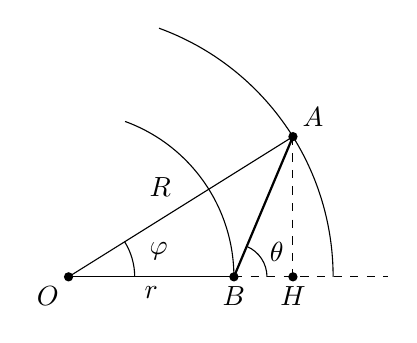
\begin{tikzpicture}[scale=1.4]
\coordinate (O) at (0,0);
\coordinate (B) at (1.5,0);
\coordinate (A) at ({2.4*cos(32)},{2.4*sin(32)});
\coordinate (H) at ({2.4*cos(32)},0);
\draw (2.4,0) arc (0:70:2.4);
\draw (1.5,0) arc (0:70:1.5);
\draw (O) -- (A) node[midway,above left]{$R$};
\draw (O) -- (B) node[midway,below]{$r$};
\draw[dashed] (B) -- (2.9,0);
\draw[dashed] (A) -- (H);
\draw[thick] (A) -- (B);
\fill (O) circle (1.2pt) node[below left]{$O$};
\fill (A) circle (1.2pt) node[above right]{$A$};
\fill (B) circle (1.2pt) node[below]{$B$};
\fill (H) circle (1.2pt) node[below]{$H$};
\draw (0.6,0) arc (0:32:0.6);
\node at ({0.85*cos(16)},{0.85*sin(16)}) {$\varphi$};
\draw (1.8,0) arc (0:67:0.3);
\node at ({1.5+0.45*cos(30)},{0.45*sin(30)}) {$\theta$};
\end{tikzpicture}

{\small Figura fora de escala: $H$ é o pé da perpendicular baixada de $A$ sobre a reta $OB$.}
\end{center}

\textbf{1. A trajetória se repete.} Em cada ponto de reflexão $P$, o raio refletido é o simétrico do raio incidente em relação à reta $OP$. Em $B$, portanto, o trecho seguinte $BA'$ é a imagem de $BA$ pela simetria em relação a $OB$, e então $\angle BOA'=\angle AOB=\varphi$. O mesmo vale em $A'$ (simetria em relação a $OA'$), e assim por diante. Além disso, a reflexão preserva a distância da reta do raio ao centro, $d=r\sin\theta<r$. Assim, todo raio que sai do espelho externo atinge o interno, e todo raio que sai do interno (que é convexo) atinge o externo. As reflexões se alternam entre os dois espelhos, cada trecho subtende o mesmo ângulo central $\varphi$, e o ângulo de incidência em todos os pontos do espelho interno é $\theta$.

\textbf{2. Condição de fechamento.} Com $n$ reflexões em cada espelho em uma volta, há $2n$ trechos, cada um de ângulo central $\varphi$. Como os raios se sobrepõem após exatamente uma volta,
\[
2n\varphi=2\pi\quad\Longrightarrow\quad \varphi=\frac{\pi}{n}.
\]

\textbf{a)} No triângulo retângulo $OHA$: $OH=R\cos\varphi$ e $AH=R\sin\varphi$. O feixe chega a $B$ vindo de fora do cilindro interno, logo $\theta<90^\circ$. Então $H$ fica no prolongamento de $OB$ além de $B$, com $BH=R\cos\varphi-r$. Como $BH$ está sobre a normal em $B$, $\theta=\angle ABH$. No triângulo retângulo $BHA$:
\[
\tan\theta=\frac{AH}{BH}=\frac{R\sin\varphi}{R\cos\varphi-r}=\frac{\sin(\pi/n)}{\cos(\pi/n)-r/R}.
\]
Com $r/R=\sqrt{3}/2$:
\[
\boxed{\tan\theta=\frac{\sin(\pi/n)}{\cos(\pi/n)-\frac{\sqrt{3}}{2}}=\frac{2\sin(\pi/n)}{2\cos(\pi/n)-\sqrt{3}}}
\]
(adimensional, como deve ser).

\textbf{b)} Para que haja reflexão de fato em $B$, o feixe precisa chegar ao espelho interno por fora e não rasante, ou seja, $0<\theta<90^\circ$. Como o numerador $\sin(\pi/n)$ é positivo, isso equivale a $\tan\theta>0$:
\[
\cos\frac{\pi}{n}>\frac{\sqrt{3}}{2}=\cos\frac{\pi}{6}
\;\Longrightarrow\;\frac{\pi}{n}<\frac{\pi}{6}
\;\Longrightarrow\; n>6 .
\]
\begin{itemize}
\item $n=6$: $\cos(\pi/6)=\sqrt{3}/2$ e $\theta=90^\circ$. A trajetória seria o hexágono regular inscrito no cilindro externo, cujo apótema é $R\cos 30^\circ=r$: os lados apenas tangenciam o cilindro interno. A incidência é rasante e não há reflexão no espelho interno, então $n=6$ deve ser excluído.
\item $n\le 5$: $\cos(\pi/n)<\sqrt{3}/2$, ou seja, $R\cos\varphi<r$. A corda que fecha o polígono passaria por dentro do cilindro interno, o que é impossível.
\end{itemize}
Para todo $n\ge 7$ existe um $\theta\in(0^\circ,90^\circ)$ que satisfaz o item a). Não há limite superior: quando $n\to\infty$, $\theta\to 0$ e o feixe fica quase radial. Conferência numérica: $n=7$ dá $\tan\theta\approx 12{,}4$ ($\theta\approx 85{,}4^\circ$, quase rasante, como esperado perto do limite); $n=12$ dá $\tan\theta\approx 2{,}59$ ($\theta\approx 68{,}9^\circ$).

Portanto $n\in\{7,8,9,\dots\}$, isto é, $n\ge 7$.

ANSWER: a) $\tan\theta=\dfrac{\sin(\pi/n)}{\cos(\pi/n)-\sqrt{3}/2}=\dfrac{2\sin(\pi/n)}{2\cos(\pi/n)-\sqrt{3}}$;\quad b) $n\in\mathbb{N}$ com $n\ge 7$ (isto é, $n=7,8,9,\dots$).%
\newpage%
\section*{Apêndice: parecer do avaliador}%
\subsection*{Questão 1: nota 9,5 (aprovada, rodada 1 de 1)}%
\textbf{Resposta da resolução às cegas do avaliador:} a) O movimento é oscilatório quando a partícula fica presa no poço de potencial em torno de x = 0, ou seja, para -2 m < x < 4 m (intervalo aberto), com energia 0 < E < 32/3 J. Os extremos ficam de fora: x = 4 m é equilíbrio instável e x = -2 m é onde Ep volta a valer 32/3 J, pois 32/3 - Ep = (x-4)$^2$(x+2)/3.\newline%
\newline%
b) E\_sup = Ep(4) = 2$\cdot$16 - 64/3 = 32/3 J $\approx$ 10,7 J. É um supremo e não um máximo: com E = 32/3 J a partícula leva tempo infinito para chegar a x = 4 e não volta, então não oscila. A faixa de energia para oscilar é 0 < E < 32/3 J.\newline%
\newline%
c) Gráfico v(t), com v$_{0}$ = $\surd$(2E/m):\newline%
{-} Em t = 0 a velocidade vale -v$_{0}$ e a tangente é horizontal, porque F(0) = 0.\newline%
{-} A velocidade sobe, com concavidade para cima, e cruza o zero em t$_{1}$, no ponto de retorno x\_A < -2 m (onde Ep(x\_A) = E). Ali a inclinação é a maior do trecho, o que gera um ponto de inflexão.\newline%
{-} Em t = 2t$_{1}$ chega a +v$_{0}$ com tangente horizontal (máximo local). O trecho de 0 a 2t$_{1}$ é simétrico em relação ao ponto (t$_{1}$, 0).\newline%
{-} Depois a velocidade cai até o mínimo positivo v\_min = $\surd$(2(E - 32/3)/m), em x = 4 m, também com tangente horizontal. Ela nunca volta a zero.\newline%
{-} Por fim, a velocidade cresce sem limite e a partícula escapa para +$\infty$. Rigorosamente, isso acontece em tempo finito: o gráfico tem uma assíntota vertical em t*.\newline%
Não há oscilação nesse caso.\par %
Conferi o enunciado no PDF e ele coincide com a transcrição. As três respostas finais coincidem com as da minha referência.\newline%
\newline%
**a)** A resposta é -2 m < x < 4 m, intervalo aberto, com 0 < E < 32/3 J. O candidato:\newline%
{-} obtém x = -2 fatorando x$^3$ - 6x$^2$ + 32 = (x-4)$^2$(x+2), reconhecendo a raiz dupla em 4;\newline%
{-} exclui os extremos com o argumento certo: perto do equilíbrio instável, E - E\_p $\approx$ 2(x-4)$^2$, então |?| $\propto$ |x-4| e a aproximação leva tempo infinito;\newline%
{-} explica por que x < -2 e x > 4 ficam de fora.\newline%
\newline%
**b)** A resposta é E\_sup = E\_p(4) = 32/3 J $\approx$ 10,7 J. A faixa 0 < E < 32/3 está correta, com E = 0 identificado como repouso.\newline%
\newline%
**c)** A descrição está completa e correta:\newline%
{-} v(0) = -$\surd$(2E/m), com tangente horizontal;\newline%
{-} um único ponto de retorno x$_{1}$ < -2;\newline%
{-} cruzamento do zero em t$_{1}$, com inflexão e inclinação máxima do trecho;\newline%
{-} simetria v(2t$_{1}$ - t) = -v(t), deduzida corretamente;\newline%
{-} máximo local +v$_{0}$ em t$_{2}$ = 2t$_{1}$;\newline%
{-} mínimo local positivo v\_min = $\surd$(2(E - 32/3)/m) em x = 4;\newline%
{-} crescimento ilimitado, com divergência em tempo finito, justificada por v $\approx$ $\surd$(2/(3m))$\cdot$x\^{}\{3/2\} e pela convergência de $\int$x\^{}\{{-}3/2\}dx.\newline%
\newline%
Integrei a equação de movimento por RK4 e os pontos do gráfico TikZ batem com a solução numérica com até 3 casas decimais.\newline%
\newline%
Todas as armadilhas foram tratadas:\newline%
{-} intervalo aberto;\newline%
{-} raiz -2;\newline%
{-} equilíbrios tirados de F = 0, e não de E\_p = 0;\newline%
{-} E\_p(4) = 32/3;\newline%
{-} v não se anula em x = 4;\newline%
{-} sinal inicial da velocidade;\newline%
{-} ausência de periodicidade;\newline%
{-} divergência em vez de um valor{-}limite.\newline%
\newline%
Restam apenas detalhes de apresentação: a assíntota não aparece desenhada, faltou dizer quais parâmetros geraram o gráfico e a concavidade e o caráter de 'supremo' ficam implícitos. A resolução tem qualidade de gabarito comentado.%
\begin{itemize}%
\item%
{[}minor{]} Item c: o esboço só vai até t $\approx$ 3,67 s (xmax = 4,1). A assíntota vertical em t\_$\infty$ fica fora da janela: numericamente t\_$\infty$ $\approx$ 4,7 s para m = 1 kg e E = 12 J. Ela aparece só no rótulo 'v$\to$+$\infty$ (em t\_$\infty$ finito)' e não é desenhada. O correto seria marcar t\_$\infty$ no eixo e desenhar uma assíntota tracejada, mesmo que fora de escala.%
\item%
{[}minor{]} O gráfico diz 'formato qualitativo, sem escala', mas é na verdade uma integração numérica exata para m = 1 kg e E = 12 J. Conferi por RK4: v$_{0}$ = 4,899, t$_{1}$ = 0,653 s, t$_{2}$ = 1,307 s, t$_{3}$ = 2,613 s e v\_min = 1,633 m/s, todos batendo com os pontos plotados. Faltou dizer quais parâmetros foram usados, já que a massa não é dada.%
\item%
{[}minor{]} O texto do item c não diz com todas as letras qual é a concavidade em cada trecho (para cima em 0 < t < t$_{1}$, para baixo perto de t$_{2}$ etc.), embora a figura mostre isso corretamente. A frase 'em t$_{1}$ a inclinação é máxima' só vale dentro do trecho {[}0, t$_{2}${]}, pois para x > 4 a inclinação fica ilimitada. Convinha explicitar esse escopo.%
\item%
{[}minor{]} Item b: a ideia de 'supremo, e não máximo' fica só implícita ('se E $\geq$ E\_p(4)\ldots{} não volta mais'). Uma frase explícita resolveria: o valor 32/3 J não pertence ao conjunto das energias que geram oscilação. O comentário 'o modelo perde validade física antes disso', no item c, é dispensável.%
\end{itemize}%
\subsection*{Questão 2: nota 9,5 (aprovada, rodada 1 de 1)}%
\textbf{Resposta da resolução às cegas do avaliador:} a) R\_A/R\_B = 16/9. b) v\_A/v\_B = 3/4. c) M\_B/M\_CA = 1/8. d) v\_B/v\_CA = 2 (v\_CA = 2v\_A/3). e) CA está no apoastro: logo após o choque frontal, a velocidade de CA é perpendicular ao raio vetor, então ele está numa apside, e ela é menor que a velocidade circular local (2v\_A/3 < v\_A). Pelo cálculo, a = 8R\_B/7 < R\_A = 16R\_B/9, r\_p = 32R\_B/63 e e = 5/9.\par %
Conferi a transcrição com o PDF (pág. 2) e ela está fiel. As respostas finais do candidato coincidem com as minhas em todos os itens, e conferi as contas com frações exatas em python. a) R\_A/R\_B = 16/9: o candidato converteu corretamente os períodos para dias terrestres (640 e 270). b) v\_A/v\_B = 3/4, verificado de duas formas. c) M\_B/M\_CA = 1/8: as porcentagens foram convertidas corretamente (razão 81/2048), a força de S sobre CA foi avaliada em R\_A e a ordem da razão está certa. d) v\_B/v\_CA = 2: a energia de CA usa a velocidade incógnita no ponto R\_A, a razão de massas do item (c) foi aplicada e o sinal está correto (E\_CA = -7/16$\cdot$M\_CA$\cdot$v\_B$^2$). O candidato não caiu na armadilha de aplicar -GMm/(2R\_A) a CA. e) Apoastro, com justificativa completa em duas partes. Primeiro, o momento linear do choque frontal tem a direção da velocidade de A, que é tangente, então a velocidade é perpendicular ao raio vetor e CA está numa apside. Segundo, v\_CA = (2/3)v\_A é menor que a velocidade circular local, então a gravidade excede a resultante centrípeta necessária. O candidato ainda confirmou com a = 8R\_B/7 < R\_A, e = 5/9 e r\_p = 32R\_B/63, todos conferidos. Cobriu todas as armadilhas relevantes. Os únicos defeitos são de redação ou explicitação: o anglicismo 'apse', não dizer que v\_CA $\neq$ 0 nem que o sentido final é irrelevante, e não citar 'mesmo corpo central' no item (a). A resolução tem qualidade de gabarito comentado.%
\begin{itemize}%
\item%
{[}minor{]} No item (e), usa o termo em inglês 'apse'. O correto em português é 'apside' (ou 'ápside'). Deveria escrever 'CA está numa apside'.%
\item%
{[}minor{]} No item (e), não diz explicitamente que v\_CA $\neq$ 0 nem que o sentido final de CA (direto ou retrógrado) não muda a conclusão. As duas coisas ficam implícitas em v\_CA = (2/3)v\_A > 0 e no fato de a direção ser tangente. Uma frase bastaria para fechar o argumento.%
\item%
{[}minor{]} A hipótese de que a 3ª lei de Kepler compara órbitas em torno do mesmo corpo central (S) e de que as massas planetárias são desprezíveis aparece só nas 'Hipóteses' gerais (M\_S ? massas). Não é mencionada no item (a). Também não diz explicitamente que r\_0 se cancela no item (c), embora isso fique visível na divisão. As duas omissões são aceitáveis, mas um gabarito comentado as tornaria explícitas.%
\end{itemize}%
\subsection*{Questão 3: nota 9,5 (aprovada, rodada 1 de 1)}%
\textbf{Resposta da resolução às cegas do avaliador:} a) d\_min = 3?/5. Com essa distância o raio em torno de B é r = 2?/5, e a tração no topo da semicircunferência vale exatamente zero (v$^2$ = g r).\newline%
b) R = ?/14. O fio afrouxa a 30$^\circ$ acima da horizontal (sin $\varphi$ = 1/2), com v$^2$ = 2g?/7. No vértice da parábola a velocidade é v?$^2$ = g?/14 e R = v?$^2$/g. O vértice fica a 11?/28 acima de B, ou seja, ?/28 abaixo de A.\par %
As respostas finais coincidem com as da minha referência, e conferi as duas: a) d\_min = 3?/5; b) $\rho$ = ?/14. A transcrição confere com o enunciado original (página 3).\newline%
\newline%
O candidato usa o raio certo depois de B (r = ? - d) e conserva a energia com justificativa (a tração é perpendicular à velocidade). A expressão geral da tração, T = mg(2d/(?-d) - 3 sin $\theta$), está certa e organiza bem os dois itens.\newline%
\newline%
No item a, a condição usada é a correta (T $\geq$ 0 no topo, ou seja, v$^2$ $\geq$ gr), o sentido da desigualdade está certo e o resultado é d $\geq$ 3?/5. O candidato ainda confere que, nesse limite, v\_topo$^2$ = gr.\newline%
\newline%
No item b, ele verifica antes que d = 3?/7 < 3?/5, então o fio afrouxa antes do topo. Encontra sin $\theta$ = 1/2 e v$^2$ = 2g?/7, decompõe a velocidade corretamente (60$^\circ$ com a horizontal, v\_x = v/2, sem trocar seno por cosseno) e calcula $\rho$ = v\_x$^2$/g = ?/14 no vértice da parábola. Refiz as contas em Python: o ápice fica em (-3$\surd$3?/14, 11?/28), a ?/28 abaixo de A, e a distância a B vale $\surd$229?/28 $\approx$ 0,540?, menor que r $\approx$ 0,571?. Tudo bate com a minha referência.\newline%
\newline%
Todas as armadilhas listadas foram evitadas. As falhas são apenas de rigor e de exposição:\newline%
{-} não explica que o topo do círculo fica sobre a barra (e por isso a trajetória é só uma semicircunferência);\newline%
{-} não diz que T decresce com $\theta$;\newline%
{-} não declara a hipótese d < ?;\newline%
{-} usa um argumento pouco preciso para mostrar que a esfera não toca a barra;\newline%
{-} não diz explicitamente que o ápice é o ponto mais alto de todo o movimento depois de B.\newline%
\newline%
É uma resolução no nível de gabarito comentado.%
\begin{itemize}%
\item%
{[}minor{]} Item a: a resolução não diz por que a questão pede só uma semicircunferência. O topo do círculo de centro B, no ponto (0, r), fica sobre a barra, e a esfera a encontra ali. O candidato diz apenas que o topo fica abaixo de A e chama isso de 'geometricamente compatível'. Deveria dizer explicitamente que o topo está sobre a barra e que por isso a esfera não pode dar a volta completa.%
\item%
{[}minor{]} Item a: falta dizer que T($\theta$) = mg(2d/(?-d) - 3 sin $\theta$) decresce com $\theta$. É isso que justifica impor T $\geq$ 0 só no topo ($\theta$ = 90$^\circ$) para garantir o fio esticado em todo o arco. A fórmula deixa isso evidente, mas o argumento não aparece escrito.%
\item%
{[}minor{]} A resolução não declara a hipótese d < ?, necessária para a esfera passar por baixo de B e para r = ? - d > 0. Também não comenta o instante em que o fio gruda (velocidade horizontal e fio vertical, portanto a velocidade é contínua). Esse ponto fica coberto só pela hipótese geral de que a tração é perpendicular à velocidade.%
\item%
{[}minor{]} Item b, verificação: a frase 'distância a B < r, logo {[}...{]} a esfera não toca a barra' mistura dois argumentos. Que a esfera não toca a barra decorre de x crescer de -2$\surd$3?/7 até -3$\surd$3?/14 < 0, não da distância a B. Também não se diz explicitamente que o ápice (11?/28) fica acima de todo o trecho circular (no máximo 2?/7) nem que depois do ápice a esfera só desce. São esses fatos que garantem que o ápice é o ponto mais alto de todo o movimento depois de B.%
\end{itemize}%
\subsection*{Questão 4: nota 9,5 (aprovada, rodada 1 de 1)}%
\textbf{Resposta da resolução às cegas do avaliador:} A malha infinita equivale a Req = R2(1+$\surd$5)/2 = 2 $\Omega$. As correntes na malha são 5 A, 8 A e 10 A, e as potências são 50 W, 128 W e 200 W nos intervalos {[}0,20), {[}20,40) e {[}40,60{]} s. As energias correspondentes são 1000 J, 2560 J e 4000 J. A energia total dissipada na malha entre t = 0 e t = 60 s é E = 7560 J ($\approx$ 7,56 kJ).\par %
Conferi a figura no original (p. 4). As três fontes têm a mesma polaridade. Da esquerda para a direita, a ordem é: ramo 1, S2, ramo 2, S1, ramo 3, S0. A escada começa com um R2 em SÉRIE e segue com um R2 em derivação. O candidato montou essa topologia corretamente. Também acertou a recorrência R = R2 + R2R/(R2+R) e descartou a raiz negativa, chegando a R = (1+$\surd$5)R2/2 = 2 $\Omega$. Conferi numericamente: a iteração converge para 2,000 $\Omega$.\newline%
\newline%
Ele deduziu explicitamente, pela tensão U entre os fios, que n ramos idênticos em paralelo equivalem a uma fonte V com resistência R1/n. Isso já implica que não há corrente circulando entre os ramos. Justificou também a ausência de transitório: o circuito é puramente resistivo. Contou apenas a dissipação na malha (I$^2$R) e tratou os três intervalos de 20 s separadamente.\newline%
\newline%
Valores obtidos em cada intervalo:\newline%
{-} Correntes: 5, 8 e 10 A.\newline%
{-} Potências: 50, 128 e 200 W.\newline%
{-} Energias: 1000, 2560 e 4000 J.\newline%
{-} Total: 7560 J.\newline%
\newline%
Esse total coincide com a minha referência, e refiz as contas em Python. Todas as armadilhas foram tratadas: a escada começa pelo resistor em série, a raiz negativa foi descartada, a topologia das chaves está certa, o paralelo dá V com R1/n e não nV, só a malha foi contada, a energia foi calculada por partes e a máxima transferência foi observada. A apresentação é clara e as verificações de unidades e coerência estão corretas. Há apenas dois deslizes menores: a redação ambígua sobre a máxima transferência ('abaixo' versus 'atingido') e a falta de um comentário sobre a convergência da escada. É uma resolução publicável como gabarito.%
\begin{itemize}%
\item%
{[}minor{]} Na verificação de 'Limite', o texto diz que a potência 'fica abaixo' da máxima transferível e, logo em seguida, que 'esse valor é atingido' no último intervalo. As duas frases se contradizem. O correto é 'não excede', ou seja, P $\leq$ V$^2$/(4R) = 200 W, com igualdade quando n = 3. Não afeta a conta.%
\item%
{[}minor{]} A recorrência da malha infinita (R = R2 + R2?R) é usada sem comentar que R é o limite das escadas finitas, nem por que a raiz positiva é o valor desse limite. Esse é o tratamento padrão em gabaritos e é aceitável. Uma linha sobre isso, ou a observação de que a iteração converge para 2 $\Omega$, deixaria o argumento completo.%
\end{itemize}%
\subsection*{Questão 5: nota 9,5 (aprovada, rodada 1 de 1)}%
\textbf{Resposta da resolução às cegas do avaliador:} a) Com m = 4 kg as reações são verticais e para cima:\newline%
{-} N\_C = 22/3 N $\approx$ 7,3 N\newline%
{-} N\_D = 200/3 N $\approx$ 66,7 N\newline%
{-} N\_E = 26 N\newline%
{-} N\_G = 26 N. É a força do dente sobre o trecho GE; sobre o trecho CG atua uma força de 26 N para baixo.\newline%
\newline%
b) m\_máx = 8,4 kg (42/5 kg). Nesse valor N\_C = 0, e o trecho CG está na iminência de tombar em torno de D.\par %
Conferi o enunciado na página 5 do PDF, e ele bate com a transcrição. As respostas do candidato coincidem com a minha referência nos dois itens, e refiz as contas em python com frações exatas.\newline%
\newline%
Item a: R\_C = 22/3 N, R\_D = 200/3 N, R\_E = 26 N e R\_G = 26 N. A soma das reações dá 100 N = (M + m)g.\newline%
\newline%
Item b: R\_C = (84 - 10m)/6 $\geq$ 0, logo m\_máx = 8,4 kg. No caso limite, R\_D = 96 N e R\_G = R\_E = 48 N, com soma 144 N.\newline%
\newline%
A modelagem é a correta de viga Gerber, e o candidato tratou todas as armadilhas que identifiquei:\newline%
{-} justifica a hiperestaticidade sem a articulação e diz que o dente não transmite momento;\newline%
{-} divide o peso da viga corretamente (48 N em x = 4 m e 12 N em x = 9 m), sem usar 60 N num trecho só;\newline%
{-} aplica a 3ª lei em G, com a carga para baixo no balanço de CG;\newline%
{-} usa os sinais certos nos momentos em relação a D e ainda confere tomando momentos em relação a C;\newline%
{-} confere o equilíbrio global sem incluir R\_G, que é força interna;\newline%
{-} no item b, diz que os vínculos são unilaterais e mostra explicitamente por que R\_D, R\_E e R\_G não geram limite (R\_D = 40 + 20m/3 > 0);\newline%
{-} descreve o mecanismo de falha: CG gira em torno de D, C se levanta e G desce.\newline%
\newline%
Os problemas que encontrei são só de redação: chamar de 'peso do trecho CD' o contrapeso, quando é o momento resultante do peso de CG em relação a D; não repetir na resposta final que as reações apontam para cima; e não ligar a figura do dente à modelagem. Nada disso afeta a física nem os resultados. A resolução tem nível de gabarito comentado.%
\begin{itemize}%
\item%
{[}minor{]} No item b, a frase 'o que segura a viga é o peso do trecho CD, que atua como contrapeso' é imprecisa. O que equilibra a carga em G é o momento resultante, em relação a D, do peso de todo o trecho CG: o trecho CD dá +36$\cdot$3 = 108 N$\cdot$m e o próprio balanço DG dá -12$\cdot$1 = -12 N$\cdot$m, totalizando 96 N$\cdot$m. A conta usa 48$\cdot$2 = 96 corretamente, então só a redação está errada. Bastaria escrever 'o momento do peso do trecho CG em relação a D'.%
\item%
{[}minor{]} Na resposta final o candidato escreve apenas 'Todas são verticais', sem dizer que as reações de C, D e E e a força do dente sobre GE apontam para cima. O sentido aparece na modelagem ('R\_G para cima', R $\geq$ 0), mas deveria constar também no quadro de respostas.%
\item%
{[}minor{]} O candidato não relaciona a figura 'Articulação' (dente em Z) com o papel de cada trecho, isto é, que CG sustenta GE pelo dente. A observação do enunciado já fixa isso, então não há erro, mas uma frase ligando a figura à modelagem deixaria a resolução mais completa.%
\end{itemize}%
\subsection*{Questão 6: nota 9,5 (aprovada, rodada 1 de 1)}%
\textbf{Resposta da resolução às cegas do avaliador:} {-} **a)** |i|\_mín = 1,25 A (= 5/4 A), em t = 0 s, quando v = -2 m/s. A corrente é i = (10 + 2,5v)/4.\newline%
{-} **b)** E\_r = 2$\cdot$(3,75)$^2$$\cdot$2 = 56,25 J, com i = 3,75 A constante de 2 a 4 s.\newline%
{-} **c)** F(5 s) = 45/16 N $\approx$ 2,81 N, para a direita (sentido de v, como na Figura 1). Nesse instante i = 3,125 A, a força magnética é 7,8125 N para a esquerda e m$\cdot$a = -5 N.\par %
Conferi o enunciado na p. 6 do PDF e a transcrição está fiel. As três respostas finais do candidato coincidem com a referência: a) 1,25 A em t = 0; b) 56,25 J; c) 45/16 N $\approx$ 2,81 N para a direita. Refiz as contas e os produtos vetoriais em python, com o triedro x para a direita, y para trás e z para cima. v$\times$B aponta para a frente, ou seja, do trilho de trás para o da frente, no mesmo sentido da corrente da fonte (A $\to$ trilho de trás $\to$ barra $\to$ trilho da frente $\to$ B). Logo a fem soma: i = (10 + 2,5v)/4. Com i saindo para a frente na barra, iL$\times$B aponta para a esquerda, e F = ma + BiL = -5 + 7,8125 = 2,8125 N. O balanço de potência fecha (34,0625 W dos dois lados).\newline%
\newline%
O candidato trata todas as armadilhas:\newline%
{-} modela a fonte com ? = 10 V e r = 2 $\Omega$;\newline%
{-} acerta o sinal da fem a partir da leitura correta da perspectiva e da polaridade (i sai de A);\newline%
{-} mostra que i fica entre 1,25 e 3,75 A, é sempre positiva e fica dentro da característica, e por isso o mínimo está em v = -2 m/s, não em v = 0;\newline%
{-} no item b conta só a energia em r;\newline%
{-} no item c inclui m$\cdot$a, usa a corrente total na força magnética e informa o sentido de F.\newline%
\newline%
A exposição é limpa e enxuta. Só há ressalvas menores:\newline%
{-} a 'verificação' não é independente;\newline%
{-} falta uma linha justificando a leitura da perspectiva;\newline%
{-} a menção a Lenz é ligeiramente imprecisa;\newline%
{-} a notação de energia pode confundir.\newline%
\newline%
É uma resolução de nível gabarito.%
\begin{itemize}%
\item%
{[}minor{]} A 'Verificação' do item c não confere nada de forma independente: só reescreve a 2ª lei de Newton (F\_m/m = 1,56 > 1 m/s$^2$). Um teste independente seria o balanço de potência em t = 5 s: Fv + ?i = (r+R)i$^2$ + m$\cdot$v$\cdot$a, que dá 34,0625 W dos dois lados. Esse balanço confirmaria ao mesmo tempo o sinal da fem e o sentido de F.%
\item%
{[}minor{]} A leitura da perspectiva ('o trilho desenhado mais acima é o de trás') aparece como afirmação, sem justificativa. Uma linha bastaria: a barra está desenhada oblíqua, indo da frente{-}esquerda para trás{-}direita, e B vertical é perpendicular ao plano horizontal dos trilhos. É dessa leitura que depende o sinal da fem, o ponto decisivo da questão.%
\item%
{[}minor{]} A frase 'Isso é coerente com Lenz: para v>0, a força freia a barra' mistura as coisas. A força BiL usa a corrente total, que é dominada pela fonte, e não só a parcela induzida. Para v<0 essa mesma força, sempre para a esquerda, acelera a barra no sentido do movimento (a fonte age como motor). O que está dito não é falso, mas atribuir a Lenz o sentido da força total é impreciso.%
\item%
{[}minor{]} Notação: o candidato usa ? para a fem e E\_r para a energia. É aceitável, mas pode confundir. W\_r ou U\_r seria mais claro.%
\end{itemize}%
\subsection*{Questão 7: nota 9,5 (aprovada, rodada 1 de 1)}%
\textbf{Resposta da resolução às cegas do avaliador:} a) V(r = a) = kQ/(2a), que é o potencial do condutor da Fig. 1.\newline%
b) Fig. 2: V(r) = kQ/|r| - kQ/(6a) para |r| $\leq$ 2a (V(a) = 5kQ/(6a)). Patamar V = kQ/(3a) para 2a $\leq$ |r| $\leq$ 3a (V(2a) = V(3a) = kQ/(3a)). V = kQ/|r| para |r| $\geq$ 3a. O gráfico é par em r, contínuo, tende a +$\infty$ quando r $\to$ 0 e a 0 no infinito.\newline%
c) Casca menor (a, 2a): superfície interna -Q, externa +4Q/5. Casca maior (2a, 3a): superfície interna -Q, externa +6Q/5. O potencial comum durante a ligação foi 2kQ/(5a), e as cargas se mantêm depois que o fio é retirado.\par %
As respostas finais coincidem com a referência em todos os itens. a) V(a) = kQ/(2a), justificado por superposição e pela equipotencialidade do condutor. b) V = kQ/r - kQ/(6a) na cavidade, kQ/(3a) no metal e kQ/r fora; V(a) = 5kQ/(6a) e V(2a) = V(3a) = kQ/(3a). O gráfico compilado é par, contínuo, tem patamar entre 2a e 3a e marca os valores pedidos. c) Superfícies internas com -Q; externas com +4Q/5 (casca menor) e +6Q/5 (casca maior); potencial comum 2kQ/(5a). Todas as armadilhas foram tratadas: Gauss no metal, conservação da carga total (q$_{1}$ + q$_{2}$ = 2Q), raios externos, hipóteses de cascas afastadas e fio desprezível, cargas mantidas após retirar o fio, e verificação do sentido da transferência. As únicas falhas são estéticas no esboço (curva cortada antes do topo do eixo, rótulo sobreposto) e a notação r em vez de |r|. A resolução tem qualidade de gabarito comentado.%
\begin{itemize}%
\item%
{[}minor{]} No gráfico TikZ, a curva da cavidade vai só de |r| = 0,75a até 2a e para em cerca de 1,17 kQ/a, abaixo do topo do eixo (ymax = 1,35). Por isso o desenho não mostra que V $\to$ +$\infty$ quando r $\to$ 0. O texto afirma a divergência, mas o desenho deveria começar perto de |r| $\approx$ 0,66a para tocar o topo, ou indicar a assíntota no eixo V.%
\item%
{[}minor{]} O rótulo 5kQ/(6a) no eixo V fica sobre a linha tracejada horizontal e encostado no ramo esquerdo da curva. É um problema estético: o gráfico continua legível.%
\item%
{[}minor{]} Os casos de V(r) estão escritos só para r > 0, embora o gráfico cubra r < 0. Os ramos negativos estão justificados pela frase 'depende só de |r|', mas escrever |r| nas expressões seria mais limpo.%
\end{itemize}%
\subsection*{Questão 8: nota 9,5 (aprovada, rodada 1 de 1)}%
\textbf{Resposta da resolução às cegas do avaliador:} a) O calor retirado do suco é Q\_F = 35 000 + 72 500 + 12 500 = 120 000 kcal = 4,8$\cdot$10$^{8}$ J. O COP de Carnot do refrigerador é 246/61,5 = 4, e o COP real é 3. O trabalho vale W = 1,6$\cdot$10$^{8}$ J em 5760 s, o que dá P $\approx$ 27,8 kW $\approx$ 37 HP (exatamente 1000/27 $\approx$ 37,04 HP).\newline%
\newline%
b) 37 HP > 30 HP, então a estimativa do engenheiro não procede: 30 HP não atende, nem "com folga". Com 30 HP o processo levaria cerca de 118,5 min, e não 96 min. Os 30 HP só bastariam para uma máquina ideal de Carnot (cerca de 27,8 HP). Perdas reais, como infiltração de calor e ineficiências, exigem potência ainda maior que 37 HP.\par %
Conferi o enunciado na página 8 do PDF original, e a transcrição está fiel. Refiz as contas em python. A resolução do candidato está correta e coincide com a minha referência em todos os itens.\newline%
\newline%
**Item a: correto, $\approx$ 37 HP**\newline%
{-} As três etapas estão presentes: 35 000 + 72 500 + 12 500 = 1,2$\cdot$10$^{5}$ kcal = 4,8$\cdot$10$^{8}$ J, usando 1 cal = 4 J como manda a prova.\newline%
{-} O COP é o de refrigerador, calculado com temperaturas absolutas: $\beta$\_C = 246/61,5 = 4. Com o fator 3/4, o COP real é $\beta$ = 3.\newline%
{-} O trabalho é W = 1,6$\cdot$10$^{8}$ J. A potência média é W/5760 s $\approx$ 27,8 kW = 1000/27 HP $\approx$ 37 HP, usando 1 HP = 0,75 kW.\newline%
{-} O candidato também calcula o calor rejeitado, Q\_Q = 6,4$\cdot$10$^{8}$ J, e confere a ordem de grandeza: 83 kW / 3 $\approx$ 28 kW.\newline%
\newline%
**Item b: correto e bem argumentado**\newline%
{-} A conclusão é explícita: 37 HP > 30 HP, logo a estimativa não procede.\newline%
{-} A diferença é quantificada: 30 HP fica 19 \% abaixo do necessário e entrega 81 \% do trabalho exigido em 96 min. O tempo com 30 HP seria $\approx$ 118,5 min. Conferi todos esses valores.\newline%
{-} O candidato observa que 37 HP é um limite inferior, porque a conta despreza a infiltração pelas paredes, a massa térmica da câmara e da embalagem e o rendimento do motor.\newline%
\newline%
**Armadilhas:** todas foram evitadas.\newline%
{-} Considerou as três etapas, incluindo o calor latente.\newline%
{-} Usou kelvin.\newline%
{-} Usou o COP de refrigerador, e não o de bomba de calor.\newline%
{-} Aplicou o fator 3/4.\newline%
{-} Usou como fontes térmicas a câmara e o ambiente.\newline%
{-} Tratou a potência como média e não a confundiu com Q\_F nem com Q\_Q.\newline%
{-} Deu uma conclusão explícita no item b.\newline%
\newline%
**Restrições:** só há detalhes menores.\newline%
{-} A igualdade 27,8/0,75 = 1000/27 mistura um valor arredondado com uma fração exata.\newline%
{-} A aproximação de 273 K não é comentada.\newline%
{-} Faltou a observação opcional de que 30 HP só bastariam para uma máquina ideal de Carnot.\newline%
\newline%
A resolução tem qualidade de gabarito comentado.%
\begin{itemize}%
\item%
{[}minor{]} A conversão para HP escreve P = 27,8/0,75 HP = 1000/27 HP. Isso iguala um quociente com valor arredondado ($\approx$ 37,07) a uma fração exata ($\approx$ 37,04). Não muda o resultado, mas o rigor pede escrever P = (1,6$\cdot$10$^{8}$/5760)/750 = 1000/27 $\approx$ 37 HP, ou usar '$\approx$' em vez de '='.%
\item%
{[}minor{]} A resolução usa 273 K (-27 $^\circ$C = 246 K; 34,5 $^\circ$C = 307,5 K) sem dizer que adota essa aproximação. Uma frase bastaria, por exemplo: com 273,15 K o COP fica $\approx$ 4,002 e o resultado não muda.%
\item%
{[}minor{]} A discussão do item b poderia ser mais completa, mas isso é opcional. Faltou dizer que os 30 HP só bastariam se a máquina fosse ideal (Carnot, $\approx$ 27,8 HP). Faltou também dizer que, para 30 HP bastarem em 96 min, o COP teria de ser $\approx$ 3,7, ou seja $\approx$ 93 \% do de Carnot, acima dos 75 \% informados. O que está na resolução já sustenta bem a conclusão.%
\end{itemize}%
\subsection*{Questão 9: nota 9,5 (aprovada, rodada 1 de 1)}%
\textbf{Resposta da resolução às cegas do avaliador:} a) I($\theta$) = I$_{1}$($\theta$)$\cdot${[}4 + 2$\surd$3$\cdot$cos(2$\pi$ a sen $\theta$/$\lambda$){]}, o que equivale a I = I$_{1}$ + 3I$_{1}$ + 2$\surd$3$\cdot$I$_{1}$$\cdot$cos(2$\pi$a sen $\theta$/$\lambda$).\newline%
\newline%
b) O primeiro máximo para $\theta$ > 0 fica em sen $\theta$ = $\lambda$/a: I\_max = (4 + 2$\surd$3)$\cdot$I$_{1}$($\theta$) = (1+$\surd$3)$^2$$\cdot$I$_{1}$($\theta$) $\approx$ 7,46$\cdot$I$_{1}$($\theta$).\newline%
\newline%
c) O primeiro mínimo para $\theta$ > 0 fica em sen $\theta$ = $\lambda$/(2a): I\_min = (4 - 2$\surd$3)$\cdot$I$_{1}$($\theta$) = ($\surd$3-1)$^2$$\cdot$I$_{1}$($\theta$) $\approx$ 0,54$\cdot$I$_{1}$($\theta$). O mínimo não é nulo.\par %
A transcrição confere com o original da página 9. As três respostas finais coincidem com a referência e foram confirmadas numericamente pela soma exata dos campos, com L = 10$^{6}$$\lambda$ e a = 3$\lambda$.\newline%
\newline%
{-} **a)** I = I$_{1}${[}4 + 2$\surd$3 cos(2$\pi$a sen $\theta$/$\lambda$){]}. O erro em relação à soma exata dos campos é de cerca de 7$\cdot$10$^{-}$$^{9}$.\newline%
{-} **b)** O primeiro máximo para $\theta$ > 0 fica em sen $\theta$ = $\lambda$/a, com I = (4+2$\surd$3)I$_{1}$ $\approx$ 7,464 I$_{1}$.\newline%
{-} **c)** O primeiro mínimo para $\theta$ > 0 fica em sen $\theta$ = $\lambda$/(2a), com I = (4-2$\surd$3)I$_{1}$ $\approx$ 0,536 I$_{1}$.\newline%
\newline%
A resolução trata todas as armadilhas:\newline%
{-} Usa a razão de amplitudes $\surd$3, e não 3.\newline%
{-} Soma amplitudes, não intensidades.\newline%
{-} A fase é 2$\pi$a sen $\theta$/$\lambda$. Usa sen $\theta$, não $\theta$ nem tg $\theta$, e justifica pela aproximação de Fraunhofer com L ? a.\newline%
{-} O sinal da fase é irrelevante, e a resolução diz isso.\newline%
{-} No item b), exclui o máximo central e usa a ordem 1.\newline%
{-} No item c), o mínimo não é nulo, e isso é explicado como ($\surd$I$_{2}$ - $\surd$I$_{1}$)$^2$.\newline%
{-} Avalia I$_{1}$ no ângulo de cada extremo.\newline%
{-} Supõe explicitamente que I$_{1}$($\theta$) varia lentamente com $\theta$.\newline%
{-} Dá as condições de existência dos extremos.\newline%
{-} Confere a dimensão da fase.\newline%
\newline%
O texto é claro e bem organizado, no nível de um gabarito comentado. Há três ressalvas pequenas:\newline%
{-} A afirmação da média ?I? = 4I$_{1}$ está escrita de forma solta.\newline%
{-} As condições de existência deveriam ser desigualdades estritas.\newline%
{-} A resolução não menciona que as fontes precisam ter a mesma polarização.%
\begin{itemize}%
\item%
{[}minor{]} A verificação ?I? = 4I$_{1}$ = I$_{1}$ + I$_{2}$ está escrita de forma solta. I$_{1}$ depende de $\theta$, e cos $\varphi$ só tem média nula em uma média local, sobre algumas franjas, com I$_{1}$ quase constante. Não é uma média espacial global sobre o anteparo. O texto deveria dizer 'média local sobre franjas'.%
\item%
{[}minor{]} As condições de existência deveriam ser estritas: a > $\lambda$ para o máximo e a > $\lambda$/2 para o mínimo. A igualdade dá $\theta$ = 90$^\circ$, direção rasante que um ponto P de um anteparo a distância finita não atinge.%
\item%
{[}minor{]} A resolução não declara que as fontes têm a mesma polarização. Essa hipótese implícita é necessária para que o termo cruzado 2$\surd$(I$_{1}$I$_{2}$)cos $\varphi$ apareça inteiro.%
\end{itemize}%
\subsection*{Questão 10: nota 9,5 (aprovada, rodada 1 de 1)}%
\textbf{Resposta da resolução às cegas do avaliador:} a) tan $\theta$ = sin($\pi$/n) / (cos($\pi$/n) - $\surd$3/2) = 2 sin($\pi$/n) / (2 cos($\pi$/n) - $\surd$3). Aqui $\theta$ é o ângulo de incidência no espelho interno, medido a partir da normal radial em B, e cada trecho AB subtende um ângulo central de $\pi$/n.\newline%
\newline%
b) Os valores possíveis são os inteiros n $\geq$ 7 (n = 7, 8, 9, \ldots{}). A condição para B ser um ponto real de reflexão é cos($\pi$/n) > $\surd$3/2. Em n = 6 o raio é rasante ($\theta$ = 90$^\circ$ e tan $\theta$ não existe). Para n $\leq$ 5, tan $\theta$ < 0, o que é impossível. Não há limite superior para n.\par %
As duas resoluções chegam às mesmas respostas finais nos dois itens, e as respostas estão corretas.\newline%
a) tan $\theta$ = sin($\pi$/n)/(cos($\pi$/n) - $\surd$3/2) = 2 sin($\pi$/n)/(2 cos($\pi$/n) - $\surd$3).\newline%
b) n $\geq$ 7.\newline%
\newline%
**Como conferi**\newline%
{-} Reli a figura no PDF original. A linha tracejada em B é radial, então $\theta$ é o ângulo de incidência no espelho interno, como o candidato assumiu.\newline%
{-} Recalculei tan $\theta$ para n = 1 a 13. Dá negativo para n $\leq$ 5, infinito em n = 6 e positivo a partir de n = 7. Os valores 12,42 (85,4$^\circ$) para n = 7 e 2,59 (68,9$^\circ$) para n = 12 conferem.\newline%
{-} Simulei o traçado de raios em Python para n = 7, 8, 10 e 12. A trajetória fecha exatamente após 2n trechos, com passo angular de 180$^\circ$/n entre um ponto de reflexão e o seguinte.\newline%
\newline%
**Armadilhas: todas tratadas**\newline%
{-} $\theta$ foi lido como o ângulo com a normal radial, e não com a tangente.\newline%
{-} São 2n trechos por volta, então $\varphi$ = $\pi$/n, e não 2$\pi$/n.\newline%
{-} O ângulo obtuso em B no triângulo OAB foi evitado de forma elegante, usando o triângulo retângulo BHA.\newline%
{-} A invariância da trajetória foi justificada pela simetria em relação a OP e pela conservação de d = r sin $\theta$ < r. Isso também garante que as reflexões se alternam entre os dois espelhos.\newline%
{-} A condição de existência 0 < $\theta$ < 90$^\circ$ leva a cos($\pi$/n) > $\surd$3/2.\newline%
{-} O caso n = 6 foi excluído com justificativa: hexágono de apótema R cos 30$^\circ$ = r e incidência rasante.\newline%
{-} Os casos n $\leq$ 5 foram excluídos.\newline%
{-} O candidato observou que não há limite superior para n ($\theta$ $\to$ 0 quando n $\to$ $\infty$).\newline%
{-} Não confundiu $\theta$ com o ângulo de incidência no espelho externo.\newline%
{-} Declarou que a figura está fora de escala.\newline%
\newline%
**Ressalvas**\newline%
Há só imprecisões menores:\newline%
{-} a afirmação de que sin($\pi$/n) > 0 falha para n = 1, embora o resultado não mude;\newline%
{-} a justificativa da exclusão de n $\leq$ 5 é vaga ('a corda que fecha o polígono');\newline%
{-} falta uma linha para mostrar que H fica além de B.\newline%
\newline%
No conjunto, o texto é claro, rigoroso e completo, com nível de gabarito comentado publicável.%
\begin{itemize}%
\item%
{[}minor{]} No item b), o candidato escreve 'Como o numerador sin($\pi$/n) é positivo'. Isso é falso para n = 1, já que sin $\pi$ = 0. O resultado não muda: n = 1 cai no caso n $\leq$ 5 (cos $\pi$ = -1 < $\surd$3/2), e tan $\theta$ = 0 também fica fora de 0 < $\theta$ < 90$^\circ$. Mesmo assim, a afirmação está incorreta como foi escrita. Bastaria dizer 'sin($\pi$/n) $\geq$ 0, e para n $\geq$ 2 é positivo' ou tratar n = 1 à parte.%
\item%
{[}minor{]} A exclusão de n $\leq$ 5 está justificada de forma vaga: 'a corda que fecha o polígono passaria por dentro do cilindro interno' não diz qual corda é essa. O argumento preciso seria assim. R cos $\varphi$ < r significa que o pé H da perpendicular por A cai dentro do disco interno, de modo que A se projeta aquém de B na normal. Então o segmento AB chega a B por dentro do cilindro interno ($\theta$ > 90$^\circ$), ou seja, cortaria o espelho interno antes de B. Outra forma: a corda AA' entre reflexões consecutivas no espelho externo tem apótema R cos($\pi$/n) < r, então a trajetória A$\to$B$\to$A' teria de 'dobrar para fora', o que um espelho convexo não permite.%
\item%
{[}minor{]} No item a), a passagem '$\theta$ < 90$^\circ$ $\Rightarrow$ H fica no prolongamento de OB além de B' aparece sem a justificativa de uma linha. A projeção de BA sobre a normal externa vale |BA| cos $\theta$ > 0, logo OH = r + |BA| cos $\theta$ > r. Não é um erro, só um salto pequeno.%
\end{itemize}%
\end{document}